\documentclass{tufte-handout}
\usepackage{graphicx}
\usepackage{tikz}
\usetikzlibrary{arrows, positioning, decorations.pathmorphing, patterns}

\begin{document}
\section{Concept}
\begin{figure}
	\resizebox{\textwidth}{!}{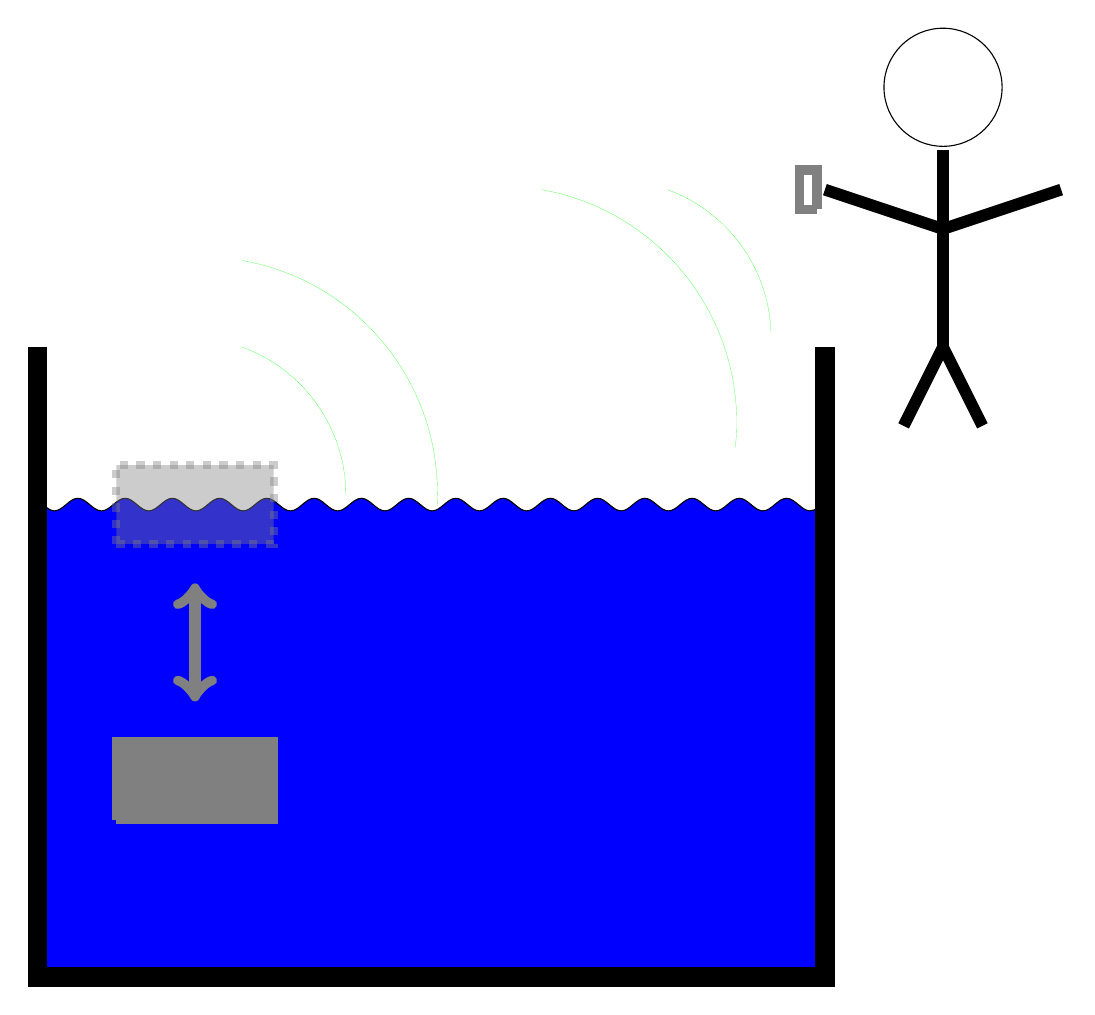
\begin{tikzpicture}
	\draw[
		decoration={
			snake,
			amplitude=0.8mm,
			segment length=6mm
		},
		fill=blue
	] decorate {(10,6) -- (0,6)} -- (0,0) -- (10,0) -- (10,6);
	\draw[
		line width=0.25cm
	] (10,8) -- (10,0) -- (0,0) -- (0,8);
	\draw[
		color=gray,
		fill=gray,
		line width=0.1cm
	] (1,2) -- (3,2) -- (3,3) -- (1,3) -- (1,2);
	\draw[
		color=black,
		line width=0.15cm
	] (11,7) -- (11.5,8) -- (12,7);
	\draw[
		color=black,
		line width=0.15cm
	] (11.5,8) -- (11.5,10.5);
	\draw[
		color=black,
		line width=0.15cm
	] (11.5, 9.5) -- (10, 10);
	\draw[
		color=black,
		line width=0.15cm
	] (11.5, 9.5) -- (13, 10);
	\node[
		circle,
		draw,
		minimum width=1.5cm,
		inner sep=0pt
	] (head) at (11.5, 11.3) {};
	\draw[
		color=gray,
		line width=0.12cm
	] (9.9,9.75) -- (9.9,10.25) -- (9.68,10.25) -- (9.68, 9.75) -- (9.9,9.75);
	\draw[
		color=gray,
		line width=0.1cm,
		fill=gray,
		opacity=0.4,
		dashed
	] (1,5.5) -- (3,5.5) -- (3,6.5) -- (1,6.5) -- (1,5.5);
	\draw[
		<->,
		line width=0.15cm,
		color=gray
	] (2,5) -- (2,3.5);
	\draw[
		color=green,
		line width=0.05
	] (2.6,8) arc (70:0:2cm);
	\draw[
		color=green,
		line width=0.05
	] (2.6,9.1) arc (80:-3:3cm);
	\draw[
		color=green,
		line width=0.05
	] (6.4,10) arc (80:-6:3cm);
	\draw[
		color=green,
		line width=0.05
	] (8,10) arc (70:2:2cm);


\end{tikzpicture}
}
	\caption{This submarine is meant to dive autonomously to the depths of the
		sea. Such dives are scheduled by an app on the smartphone of the user and
		the data that is gathered by the submarine is reported back to the
		smartphone and appealingly presented to the user.}
\end{figure}
The goal of this project is to build a self-contained low-cost submarine that
can dive autonomously and gather data from the water it dives in. In order to
communicate with this submarine a bluetooth connection with a smartphone is
used. The software for the submarine as well as the android app are provided
under an open source license, please refer to
\url{https://github.com/weltoph/submarine} for the details.
\section{Submarine}
\begin{figure}
	\resizebox{\textwidth}{!}{\input{../presentation/tikz/subsketch.tex}}
	\caption{This is a sketch of how to construct a submarine.}
\end{figure}
The submarine construction is in the following separated in two parts, namely
in the construction of the dive tank which is the most crucial part of building
a submarine and some general notes on further steps.

\subsection{Dive Tank}
As starting point we use a syringe which is very easy to obtain by any
pharmacy. The biggest size we found is about 100 ml. Furthermore we used a
Nema17 stepper motor for the necessary movements. In order to operate the
stepper motor from the arduino we relied on an EasyDriver\footnote{Please refer
to the excellent documentation at
\url{http://www.schmalzhaus.com/EasyDriver/}}.
Now, in order to translate the rotation of the stepper motor to a push-pull
movement to pull out and push in the plunger of the syringe we attach a
threaded rod with a shaft coupling on the stepper motor. The rotation is
translated to the needed push-pull movement by countersinking a nut (protected
against roatation) in the long end of the plunger\footnote{\centering
\resizebox{0.2\textwidth}{!}{\includegraphics{../presentation/pic/second-divetank}}
\\The location of the nut is marked here.}.
Screwing the threaded rod in
the nut translates to a lifting motion since the nut cannot rotate itself. The
rotation direction of the threaded rod controls the direction of the lifting
motion. In order to connect the syringe to the stepper motor we used threading
rods and nuts (see the picture above).

\subsection{Further notes}
Another crucial aspect of building a submarine is finding a hull that is
leakproof. We used PVC tubes that are actually used as pipes for fluids and
thus are equipped with seals. This gives a leakproof hull but on the other hand
the used PVC is especially designed for resistance. Permanently attaching
something to those tubes is therefore complicated. Glueing stuff on these tubes
is very difficult; therefore, we advocate solutions with more physical quality.
For the dive tank the threaded rods that connect stepper motor and syringe
can be chosen long enough such that they overtop the length of the syringe.
Then the syringe can be fixed to the hull by screwing three parallel holes in
the lid of the tube, the middle for the tip of the syringe and the outer holes
for the threaded rods. Then the whole dive tank can be attached to the lid with
nuts applied to the threaded rods. Of course it is also necessary to leakproof
all holes screwed in the hull. Silicone is your best friend for this situation!
This also applies to all sensors that lead to the outside.

It is also important to mind the volume of your constructed submarine. Volume leads to
uplift which has to be tarn with weight to enable dives. Managing the volume is
therefore another important thing in the construction. Plan carefully where to
put your arduino and the sensors. The robustness of the dives of your submarine
relies heavily on the ratio of the volume of your submarine and the volume of
your dive tank. We therefore want to point out this
video\footnote{\url{https://www.youtube.com/watch?v=UmaaA-Z342A}} of our
prototype, where you can see the amount of weights that are necessary to make a
dive possible.

\section{Further Help}
This can be merely a starting point for the construction of your very own
submarine but we would be amazed if we can get anyone interested in this topic.
Furthermore we will be equally amazed if you contribute to this manual with own
experiences and discussions.
For further reference we would like to point to
\url{https://media.ccc.de/v/32c3-7265-maritime_robotics} as well as
\url{https://hackaday.io/list/7359-waterborne-projects}.

\end{document}
